\documentclass[11pt]{article}
\usepackage{amsmath,amssymb,amsmath,amsthm,amsfonts}
\usepackage{latexsym,graphicx}
\usepackage{fullpage,color}
\usepackage{url}
\usepackage[pdftex,bookmarks,colorlinks=true,citecolor=blue]{hyperref}
\usepackage{natbib}
\usepackage{graphicx,subfigure}
\usepackage{algorithm}
\usepackage{algorithmic}
\usepackage{listings}
\usepackage[dvipsnames]{xcolor}
\usepackage{color}
\usepackage{wrapfig}

\numberwithin{equation}{section}

\pagestyle{plain}

\setlength{\oddsidemargin}{0in}
\setlength{\topmargin}{0in}
\setlength{\textwidth}{6.5in}
\setlength{\textheight}{8.5in}

\newtheorem{fact}{Fact}[section]
\newtheorem{question}{Question}[section]
\newtheorem{lemma}{Lemma}[section]
\newtheorem{theorem}[lemma]{Theorem}
\newtheorem{assumption}[lemma]{Assumption}
\newtheorem{corollary}[lemma]{Corollary}
\newtheorem{prop}[lemma]{Proposition}
\newtheorem{claim}{Claim}[section]
\newtheorem{remark}{Remark}[section]
\newtheorem{definition}{Definition}[section]
\newtheorem{prob}{Problem}[section]
\newtheorem{conjecture}{Conjecture}[section]
\newtheorem{property}{Property}[section]

\def\A{{\bf A}}
\def\a{{\bf a}}
\def\B{{\bf B}}
\def\bb{{\bf b}}
\def\C{{\bf C}}
\def\c{{\bf c}}
\def\D{{\bf D}}
\def\d{{\bf d}}
\def\E{{\bf E}}
\def\e{{\bf e}}
\def\F{{\bf F}}
\def\f{{\bf f}}
\def\g{{\bf g}}
\def\h{{\bf h}}
\def\G{{\bf G}}
\def\H{{\bf H}}
\def\I{{\bf I}}
\def\K{{\bf K}}
\def\k{{\bf k}}
\def\LL{{\bf L}}
\def\M{{\bf M}}
\def\m{{\bf m}}
\def\N{{\bf N}}
\def\n{{\bf n}}
\def\PP{{\bf P}}
\def\pp{{\bf p}}
\def\Q{{\bf Q}}
\def\q{{\bf q}}
\def\R{{\bf R}}
\def\rr{{\bf r}}
\def\S{{\bf S}}
\def\s{{\bf s}}
\def\T{{\bf T}}
\def\tt{{\bf t}}
\def\U{{\bf U}}
\def\u{{\bf u}}
\def\V{{\bf V}}
\def\v{{\bf v}}
\def\W{{\bf W}}
\def\w{{\bf w}}
\def\X{{\bf X}}
\def\x{{\bf x}}
\def\Y{{\bf Y}}
\def\y{{\bf y}}
\def\Z{{\bf Z}}
\def\z{{\bf z}}
\def\0{{\bf 0}}
\def\1{{\bf 1}}



\def\AM{{\mathcal A}}
\def\CM{{\mathcal C}}
\def\DM{{\mathcal D}}
\def\EM{{\mathcal E}}
\def\GM{{\mathcal G}}
\def\FM{{\mathcal F}}
\def\IM{{\mathcal I}}
\def\JM{{\mathcal J}}
\def\KM{{\mathcal K}}
\def\LM{{\mathcal L}}
\def\NM{{\mathcal N}}
\def\OM{{\mathcal O}}
\def\PM{{\mathcal P}}
\def\SM{{\mathcal S}}
\def\TM{{\mathcal T}}
\def\UM{{\mathcal U}}
\def\VM{{\mathcal V}}
\def\WM{{\mathcal W}}
\def\XM{{\mathcal X}}
\def\YM{{\mathcal Y}}
\def\RB{{\mathbb R}}
\def\RBmn{{\RB^{m\times n}}}
\def\EB{{\mathbb E}}
\def\PB{{\mathbb P}}

\def\TX{\tilde{\bf X}}
\def\TA{\tilde{\bf A}}
\def\tx{\tilde{\bf x}}
\def\ty{\tilde{\bf y}}
\def\TZ{\tilde{\bf Z}}
\def\tz{\tilde{\bf z}}
\def\hd{\hat{d}}
\def\HD{\hat{\bf D}}
\def\hx{\hat{\bf x}}
\def\nysA{{\tilde{\A}_c^{\textrm{nys}}}}

\def\alp{\mbox{\boldmath$\alpha$\unboldmath}}
\def\bet{\mbox{\boldmath$\beta$\unboldmath}}
\def\epsi{\mbox{\boldmath$\epsilon$\unboldmath}}
\def\etab{\mbox{\boldmath$\eta$\unboldmath}}
\def\ph{\mbox{\boldmath$\phi$\unboldmath}}
\def\pii{\mbox{\boldmath$\pi$\unboldmath}}
\def\Ph{\mbox{\boldmath$\Phi$\unboldmath}}
\def\Ps{\mbox{\boldmath$\Psi$\unboldmath}}
\def\ps{\mbox{\boldmath$\psi$\unboldmath}}
\def\tha{\mbox{\boldmath$\theta$\unboldmath}}
\def\Tha{\mbox{\boldmath$\Theta$\unboldmath}}
\def\muu{\mbox{\boldmath$\mu$\unboldmath}}
\def\Si{\mbox{\boldmath$\Sigma$\unboldmath}}
\def\si{\mbox{\boldmath$\sigma$\unboldmath}}
\def\Gam{\mbox{\boldmath$\Gamma$\unboldmath}}
\def\Lam{\mbox{\boldmath$\Lambda$\unboldmath}}
\def\De{\mbox{\boldmath$\Delta$\unboldmath}}
\def\Ome{\mbox{\boldmath$\Omega$\unboldmath}}
\def\Pii{\mbox{\boldmath$\Pi$\unboldmath}}
\def\varepsi{\mbox{\boldmath$\varepsilon$\unboldmath}}
\newcommand{\ti}[1]{\tilde{#1}}
\def\Ncal{\mathcal{N}}
\def\argmax{\mathop{\rm argmax}}
\def\argmin{\mathop{\rm argmin}}

\def\ALG{{\AM_{\textrm{col}}}}

\def\mean{\mathsf{mean}}
\def\std{\mathsf{std}}
\def\orth{\mathsf{orth}}
\def\var{\mathsf{var}}
\def\sgn{\mathsf{sgn}}
\def\tr{\mathsf{tr}}
\def\rk{\mathrm{rank}}
\def\nnz{\mathsf{nnz}}
\def\st{\mathsf{s.t.}}
\def\vect{\mathsf{vec}}
\def\sech{\mathrm{sech}}
\def\sigmoid{\mathsf{sigmoid}}
\def\din{{d_{\textrm{in}}}}
\def\dout{{d_{\textrm{out}}}}


\newcommand{\red}[1]{{\color{red}#1}}
\newcommand{\blue}[1]{{\color{blue}#1}}
\newcommand{\green}[1]{{\color{green}#1}}



\def\argmax{\mathop{\rm argmax}}
\def\argmin{\mathop{\rm argmin}}

\newenvironment{note}[1]{\medskip\noindent \textbf{#1:}}%
        {\medskip}


\newcommand{\etal}{{\em et al.}\ }
\newcommand{\assign}{\leftarrow}
\newcommand{\eps}{\epsilon}




\lstset{ %
extendedchars=false,            % Shutdown no-ASCII compatible
language=Python,                % choose the language of the code
xleftmargin=1em,
xrightmargin=1em,
basicstyle=\footnotesize,    % the size of the fonts that are used for the code
tabsize=3,                            % sets default tabsize to 3 spaces
numbers=left,                   % where to put the line-numbers
numberstyle=\tiny,              % the size of the fonts that are used for the line-numbers
stepnumber=1,                   % the step between two line-numbers. If it's 1 each line
                                % will be numbered
numbersep=5pt,                  % how far the line-numbers are from the code   %
keywordstyle=\color[rgb]{0,0,1},                % keywords
commentstyle=\color[rgb]{0.133,0.545,0.133},    % comments
stringstyle=\color[rgb]{0.627,0.126,0.941},      % strings
backgroundcolor=\color{white}, % choose the background color. You must add \usepackage{color}
showspaces=false,               % show spaces adding particular underscores
showstringspaces=false,         % underline spaces within strings
showtabs=false,                 % show tabs within strings adding particular underscores
frame=single,                 % adds a frame around the code
%captionpos=b,                   % sets the caption-position to bottom
breaklines=true,                % sets automatic line breaking
breakatwhitespace=false,        % sets if automatic breaks should only happen at whitespace
%title=\lstname,                 % show the filename of files included with \lstinputlisting;
%                                % also try caption instead of title
mathescape=true,escapechar=?    % escape to latex with ?..?
escapeinside={\%*}{*)},         % if you want to add a comment within your code
%columns=fixed,                  % nice spacing
%morestring=[m]',                % strings
%morekeywords={%,...},%          % if you want to add more keywords to the set
%    break,case,catch,continue,elseif,else,end,for,function,global,%
%    if,otherwise,persistent,return,switch,try,while,...},%
}


\begin{document}

%\setlength{\fboxrule}{.5mm}\setlength{\fboxsep}{1.2mm}
%\newlength{\boxlength}\setlength{\boxlength}{\textwidth}
%\addtolength{\boxlength}{-4mm}


\title{BackPropagation for Fully-Connected and \\Convolutional Neural Networks}

\author{\textbf{Shusen Wang} \\ Stevens Institute of Technology}

%\date{ }

\maketitle

\begin{abstract}
First, define a fully-connected (FC) layer.
Second, derive the gradients using chain rule for one FC layer.
Third, connect multiple FC layers to build a FC neural network.
Fourth, perform backpropagation using the chain rule.
Fifth, express convolution as a matrix multiplication.
Last, derive gradients for convolutional layer.
\end{abstract}


\section{Fully-Connected (FC) Layer}



We consider one fully-connected (FC) layer and follow the convention of PyTorch.
Let $\din$ be the input shape, $\dout$ be the output shape, and $b$ be the batch size.
Let $\X \in \RB^{b\times \din}$ be a batch of input vectors, $\W \in \RB^{\dout \times \din}$ be the weight matrix, and $\Z = \X \W^T \in \RB^{b\times \dout}$.
The output of this FC layer is $\X' = \sigma (\Z) \in \RB^{b\times \dout}$ where $\sigma$ is an activation function that applies elementwisely.
For example, if the activation function is ReLU, then the $(i,j)$-th entry of $\X'$ is
\begin{equation*}
    x_{ij}'
    \: = \:
    \left\{
    \begin{array}{cc}
         z_{ij}, & \textrm{if } z_{ij} > 0;  \\
         0, & \textrm{otherwise.} \\
    \end{array}
    \right.
\end{equation*}
The structure of a FC layer is illustrated in Figure~\ref{fig:differential}(left).



\section{Differentiation for FC Layer} \label{sec:differential}

Let $Q$ be the loss function that depends on $\X'$.
Suppose we know $\frac{\partial \, Q}{ \partial \, \X'} \in \RB^{b\times \dout}$ (the derivative of $Q$ w.r.t.\ $\X'$).
Since $\X$ and $\W$ influence $Q$ via $\X'$:
\begin{equation*}
    \left.
    \begin{array}{c c}
         \cdots \: \longrightarrow \: \cdots \: \longrightarrow \: & \X   \\
         & \W
    \end{array}
    \right\}
    \: \xrightarrow{\textsf{~multiply~}}  \: 
    \Z 
    \: \xrightarrow{\textsf{activation}}  \: 
    \X'
    \: \longrightarrow \: 
    \cdots
    \: \longrightarrow \: 
    Q ,
\end{equation*}
we can let the gradient flow to $\X$ and $\W$ in the opposite direction:
\begin{equation*}
    \left.
    \begin{array}{c c}
         \cdots \: \longleftarrow \: \cdots \: \longleftarrow \: & \frac{\partial \, Q }{\partial \, \X}    \\
         & \frac{\partial \, Q }{\partial \, \W} 
    \end{array}
    \right\}
    \: \longleftarrow \: 
    \frac{\partial \, Q }{\partial \, \Z} 
    \: \longleftarrow \: 
    \frac{\partial \, Q }{\partial \, \X'} .
\end{equation*}
In the following, we compute $\frac{\partial \, Q}{ \partial \, \Z}$ and then $\frac{\partial \, Q}{ \partial \, \X}$ and $\frac{\partial \, Q}{ \partial \, \W}$. 

\paragraph{From $\X'$ to $\Z$.}
First, compute $\frac{\partial \, Q}{ \partial \, \Z}  \in \RB^{b\times \dout}$.
If $\X' = \textsf{ReLU} (\Z)$,\footnote{$[\textsf{ReLU} (\Z)]_{ij} = \max \{z_{ij} , \, 0 \}$.}
then the $(i,j)$-th entry of $\frac{\partial \, Q}{ \partial \, \Z} $ is
\begin{equation*}
    \Big[\frac{\partial \, Q}{ \partial \, \Z} \Big]_{ij}
    \: = \: \frac{\partial \, Q}{ \partial \, z_{ij}}
    \: = \:  \frac{\partial \, x_{ij}' }{ \partial \, z_{ij}} \,  \frac{\partial \, Q}{ \partial \, x_{ij}'}
    \: = \: 
    \left\{
    \begin{array}{cc}
         \tfrac{\partial \, Q}{ \partial \, x_{ij}'}, & \textrm{if } z_{ij} > 0;  \\
         0, & \textrm{otherwise.} \\
    \end{array}
    \right.
\end{equation*}
Let $\A \in \RB^{b\times \dout}$ be such as matrix that 
\begin{equation*}
    a_{ij} 
    \: = \: 
    \left\{
    \begin{array}{cc}
         1, & \textrm{if } z_{ij} > 0;  \\
         0, & \textrm{otherwise.} \\
    \end{array}
    \right.
\end{equation*}
Let ``$\circ $'' denote the Hadamard product (also known as elementwise product.)
Then
\begin{equation} \label{eq:grad_q_z}
    \frac{\partial \, Q}{ \partial \, \Z}
    \: = \: \A \circ  \frac{\partial \, Q}{ \partial \, \X'}
    \: \in \: \RB^{b\times \dout} .
\end{equation}

\paragraph{From $\Z$ to $\X$.}
Second, compute $\frac{\partial \, Q}{ \partial \, \X}  \in \RB^{b\times \din}$.
Let $\x_{i:} \in \RB^{1\times \din}$ and $\z_{i:} \in \RB^{1\times \dout}$ be the $i$-th rows of $\X$ and $\Z$, respectively, for $i = 1$ to $b$.\footnote{To calculate gradient in the standard way, we must use column vectors.}
Thus $\x_{i:}^T \in \RB^{\din \times 1}$ and $\z_{i:}^T \in \RB^{ \dout \times 1}$ are the $i$-th column of $\X^T \in \RB^{\din \times b}$ and $\Z^T \in \RB^{\dout \times b}$, respectively.
It follows from the chain rule that
\begin{equation*}
    \frac{ \partial \, Q }{ \partial \, \x_{i:}^T }
    \: = \: \sum_{j=1}^{b} \frac{ \partial \, \z_{j:}^T  }{ \partial \, \x_{i:}^T } \frac{ \partial \, Q }{ \partial \, \z_{j:}^T } 
    \: = \: \frac{ \partial \, \z_{i:}^T  }{ \partial \, \x_{i:}^T } \, \frac{ \partial \, Q }{ \partial \, \z_{i:}^T } 
    + \sum_{i\neq j} \frac{ \partial \, \z_{j:}^T  }{ \partial \, \x_{i:}^T } \frac{ \partial \, Q }{ \partial \, \z_{j:}^T } .
\end{equation*}
If $i \neq j$, $\z_{j:}$ will not depend on $\x_{i:}$, and thus $\frac{ \partial \, \z_{j:}^T  }{ \partial \, \x_{i:}^T } $ is the all-zero matrix.
It follows that
\begin{equation*}
    \frac{ \partial \, Q }{ \partial \, \x_{i:}^T }
    \: = \: \underbrace{\frac{ \partial \, \z_{i:}^T  }{ \partial \, \x_{i:}^T }}_{\din \times \dout} \, 
    \underbrace{\frac{ \partial \, Q }{ \partial \, \z_{i:}^T } }_{\dout\times 1}
    \: \in \: \RB^{\din \times 1}.
\end{equation*}
Since $\z_{i:} = \x_{i:} \W^T$, we have $\z_{i:}^T = \W \x_{i:}^T$, and thus $\frac{ \partial \, \z_{i:}^T }{ \partial \, \x_{i:}^T } = \W^T  \in  \RB^{\din \times \dout }$.
It follows that
\begin{equation*}
    \frac{ \partial \, Q }{ \partial \, \x_{i:}^T }
    \: = \: \W^T \, \cdot \, \frac{ \partial \, Q }{ \partial \, \z_{i:}^T } 
    \: \in \: \RB^{\din \times 1}.
\end{equation*}
Since $\x_{i:}^T$ is the $i$-th column of $\X^T \in \RB^{\din \times b}$,
\begin{equation*}
    \frac{ \partial \, Q }{ \partial \, \X^T }
    \: = \: \Big[ \frac{ \partial \, Q }{ \partial \, \x_{1:}^T } , \; \cdots , \; \frac{ \partial \, Q }{ \partial \, \x_{b:}^T } \Big]
    \: = \: \W^T \, \cdot \, \Big[ \frac{ \partial \, Q }{ \partial \, \z_{1:}^T } , \; \cdots , \; \frac{ \partial \, Q }{ \partial \, \z_{b:}^T } \Big]
    \: = \: \underbrace{\W^T}_{\din\times \dout} \, \cdot \,  
    \underbrace{\frac{ \partial \, Q }{ \partial \, \Z^T } }_{\dout \times b}
    \: \in \: \RB^{\din \times b}.
\end{equation*}
Hence
\begin{equation} \label{eq:grad_q_x}
    \frac{ \partial \, Q }{ \partial \, \X }
    \: = \: \bigg( \frac{ \partial \, Q }{ \partial \, \X^T } \bigg)^T
    \: = \: \frac{ \partial \, Q }{ \partial \, \Z } \, \cdot \, \W
    \: \in \: \RB^{b \times \din}.
\end{equation}


\paragraph{From $\Z$ to $\W$.}
Third, compute $\frac{\partial \, Q}{ \partial \, \W}  \in \RB^{\dout\times \din}$.
Let $\z_{:j} \in \RB^{b\times 1}$ be the $j$-th columns of $\Z$
and $\w_{j:} \in \RB^{1\times \din}$ be the $j$-th row of $\W$, for $j = 1$ to $\dout$.
Thus $\w_{j:}^T \in \RB^{\din \times 1}$ is the $j$-th column of $\W^T \in \RB^{\din \times \dout}$.
It follows from the chain rule that
\begin{equation*}
    \frac{ \partial \, Q }{ \partial \, \w_{j:}^T }
    \: = \: \sum_{i=1}^{\dout} \frac{ \partial \, \z_{:i}  }{ \partial \, \w_{j:}^T } \, \frac{ \partial \, Q }{ \partial \, \z_{:i} } 
    \: = \: \frac{ \partial \, \z_{:j}  }{ \partial \, \w_{j:}^T } \, \frac{ \partial \, Q }{ \partial \, \z_{:j} } 
    + \sum_{i\neq j} \frac{ \partial \, \z_{:i}  }{ \partial \, \w_{j:}^T } \, \frac{ \partial \, Q }{ \partial \, \z_{:i} } 
    \: = \: \underbrace{ \frac{ \partial \, \z_{:j}  }{ \partial \, \w_{j:}^T } }_{\din \times b} 
    \,  \underbrace{ \frac{ \partial \, Q }{ \partial \, \z_{:j} } }_{b\times 1}
    \: \in \: \RB^{\din \times 1}.
\end{equation*}
Since $\z_{:j} = \X \w_{j:}^T \in \RB^{b\times 1}$, we can show that $\frac{ \partial \, \z_{:j} }{ \partial \, \w_{j:}^T } = \X^T \in  \RB^{\din \times b}$.
Thus
\begin{equation*}
    \frac{ \partial \, Q }{ \partial \, \w_{j:}^T }
    \: = \: \X^T  \, \cdot \,  \frac{ \partial \, Q }{ \partial \, \z_{:j} }
    \: \in \: \RB^{\din \times 1}.
\end{equation*}
Note that $\w_{j:}^T $ is the $j$-th column of $\W^T \in \RB^{\din \times \dout}$.
It follows that
\begin{equation*}
    \frac{ \partial \, Q }{ \partial \, \W^T }
    \: = \: \Big[ \frac{ \partial \, Q }{ \partial \, \w_{1:}^T } , \; \cdots , \;  \frac{ \partial \, Q }{ \partial \, \w_{\dout:}^T } \Big]
    \: = \:  \X^T  \Big[\frac{ \partial \, Q }{ \partial \, \z_{:1} } , \; \cdots , \; 
    \frac{ \partial \, Q }{ \partial \, \z_{:\dout} } \Big]
    \: = \: \underbrace{\X^T}_{\din \times b} \, \underbrace{ \frac{\partial \, Q }{ \partial \, \Z }}_{b\times \dout}
    \: \in \: \RB^{\din \times \dout} .
\end{equation*}
Hence,
\begin{equation} \label{eq:grad_q_w}
    \frac{ \partial \, Q }{ \partial \, \W }
    \: = \: \bigg( \frac{ \partial \, Q }{ \partial \, \W^T } \bigg)^T
    \: = \: \bigg( \frac{\partial \, Q }{ \partial \, \Z } \bigg)^T  \X 
    \: \in \: \RB^{\dout \times \din}.
\end{equation}


\begin{figure}[!h]
	\centering
	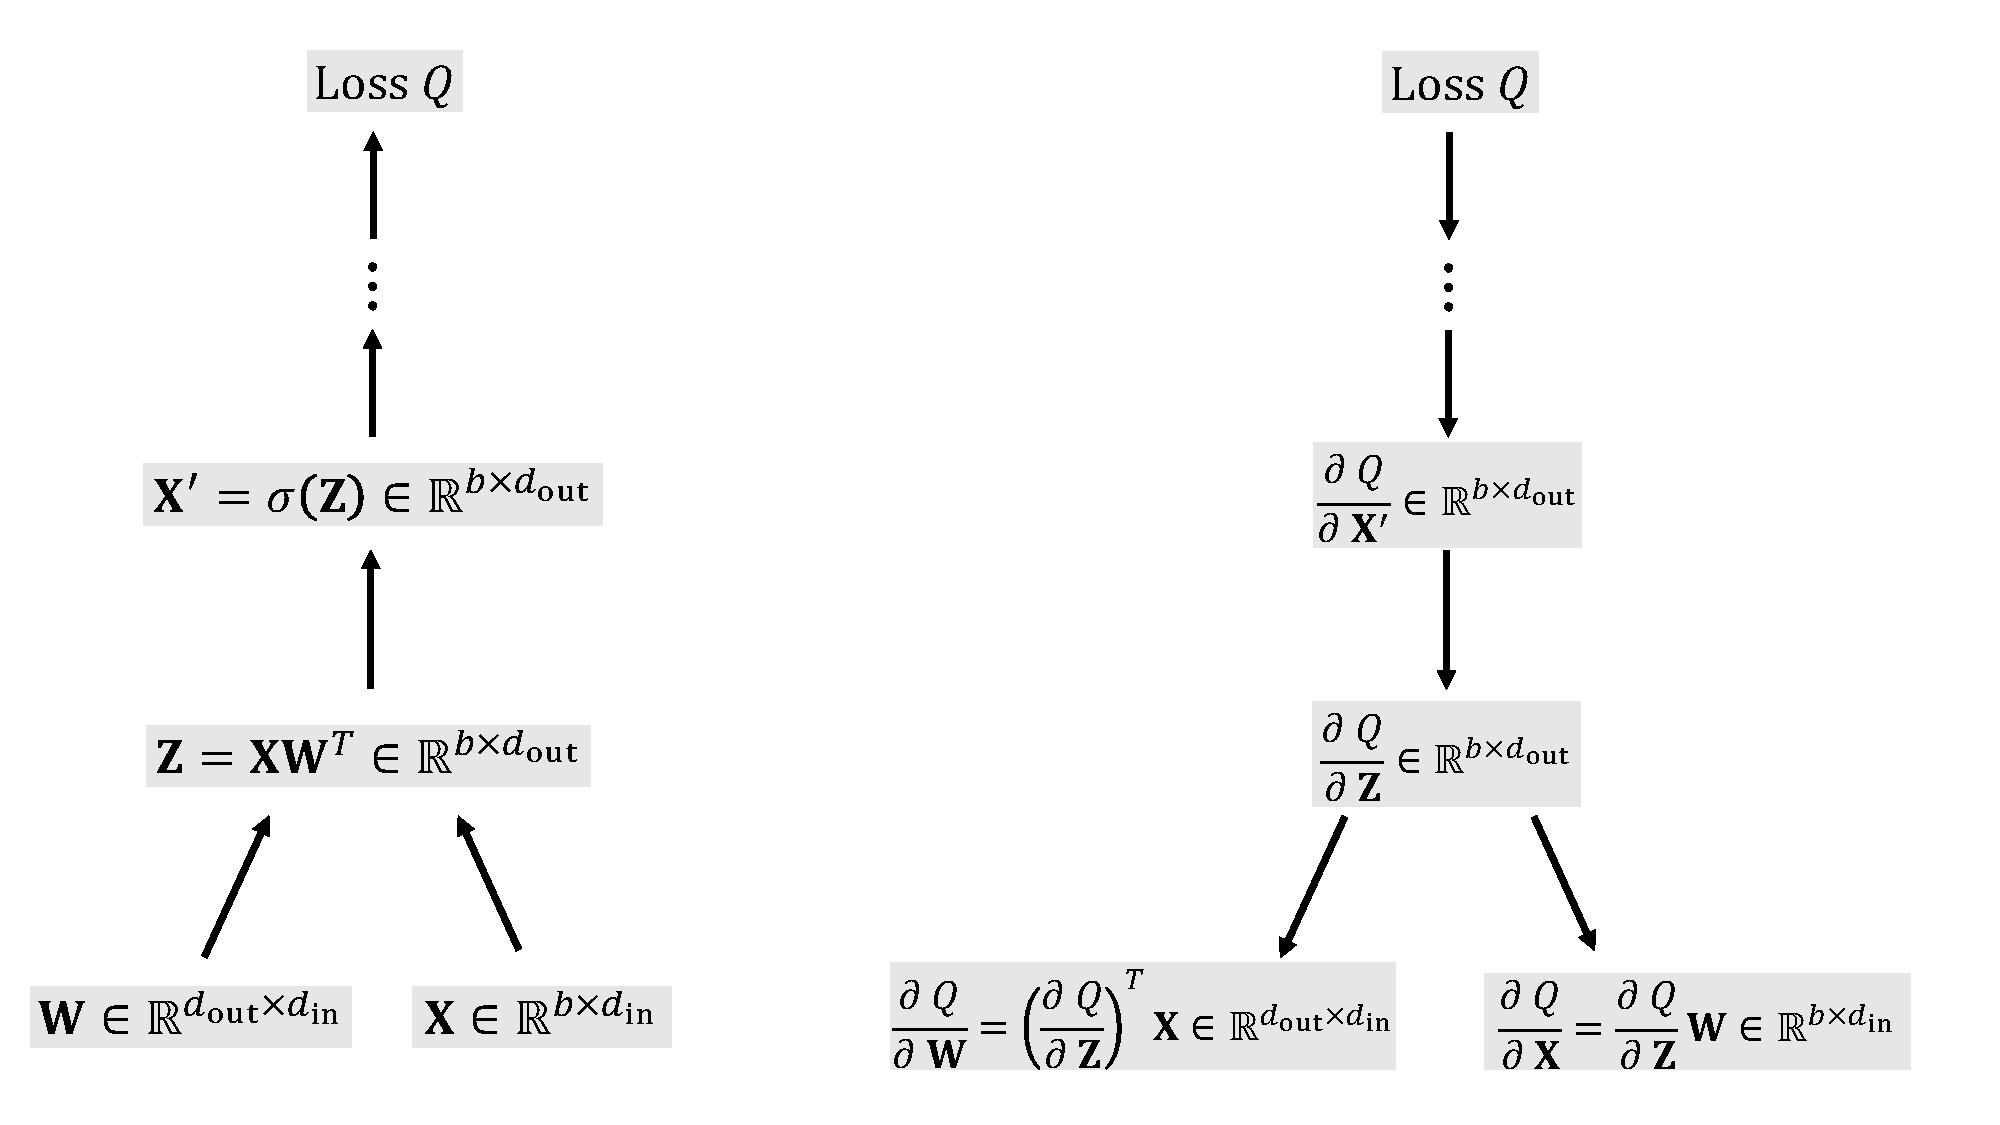
\includegraphics[width=0.85\linewidth]{figures/differential.pdf}
	\caption{Differential for one FC Layer.}
	\label{fig:differential}
\end{figure}




We summarize the gradients flow in Figure~\ref{fig:differential}.
Given $ \frac{\partial \, Q }{ \partial \, \X' }$, we can compute first $ \frac{\partial \, Q }{ \partial \, \Z }$ according to \eqref{eq:grad_q_z} and then $ \frac{\partial \, Q }{ \partial \, \X }$ according to \eqref{eq:grad_q_x} and $ \frac{\partial \, Q }{ \partial \, \W }$ according to \eqref{eq:grad_q_w}.



\section{Fully-Connected (FC) Neural Network}

An FC neural network is composed of multiple FC layers.
Suppose the FC network has $L$ ($> 1$) layers; the $l$-th layer is parameterized by weight matrix $\W^{(l)}$.
The $l$-th layer takes matrix $\X^{(l)}$ as input,
computes $\Z^{(l)} = \X^{(l)} {\W^{(l)}}^T$,
and outputs $\X^{(l+1)} = \sigma (\Z^{(l)})$.
The dependence can be depicted as
\begin{small}
\begin{equation*}
    \begin{array}{c}
         \textsf{input} \: \longrightarrow \:  \cdots \: \longrightarrow   \\
         ~
    \end{array}
    \underbrace{
    \left.
    \begin{array}{c}
         \X^{(l)}   \\
         \W^{(l)} \\
    \end{array}
    \right\}
    \: \longrightarrow \: 
    \Z^{(l)}
    \: \longrightarrow \: 
    \X^{(l+1)} }_{\textsf{the } l\textsf{-th layer}} 
    \: \longrightarrow \: 
    \cdots
    \: \longrightarrow \: 
    \X^{(L+1)} (\textsf{i.e.\ output})
    \: \longrightarrow \: 
    \textsf{loss}.
\end{equation*}
\end{small}%
Note that for $\X^{(1)} , \cdots , \X^{(L+1)}$ all have $b$ rows, where $b$ is the batch size;
but they can have different numbers of columns.\footnote{In the case of MNIST hand-written digit classification, the inputs are $784$ ($=28\times 28$) dimensional vectors, and the outputs are a $10$-dimensional vectors (for there are $10$ classes).
So $\X^{(1)}$ has $784$ columns, and $\X^{(L+1)}$ has $10$ columns.}

The $L$-th layer is called the output layer.
The output of the $L$-th layer, denote $\X^{(L+1)} \in \RB^{b\times m}$, is the prediction the neural network makes for the input $\X^{(1)}$.
Let $\Y \in \RB^{b\times m}$ be the labels of this batch of samples.\footnote{In the case of housing price prediction, the labels (housing price) are scalars, so $m=1$. In the case of hand-written digit classification, there are ten classes, and the labels are one-hot encode ($10$-dimensional vectors); thus $m=10$.}
We need to define a loss function $Q$ that measures the difference between the prediction and the ground truth (labels).
For example, the loss function can be
\begin{equation*}
    Q \left( \X^{(1)} , \Y ; \, \W^{(1)}, \cdots , \W^{(L)} \right)
    \; = \; \frac{1}{2} \Big\| \X^{(L+1)} \, - \, \Y  \Big\|_F^2 .
\end{equation*}
See Figure~\ref{fig:bp}(left) for the structure of the FC neural network (with $\Z$'s abbreviated.)




% \begin{wrapfigure}{r}{0.65\textwidth}
% 	\centering
% 	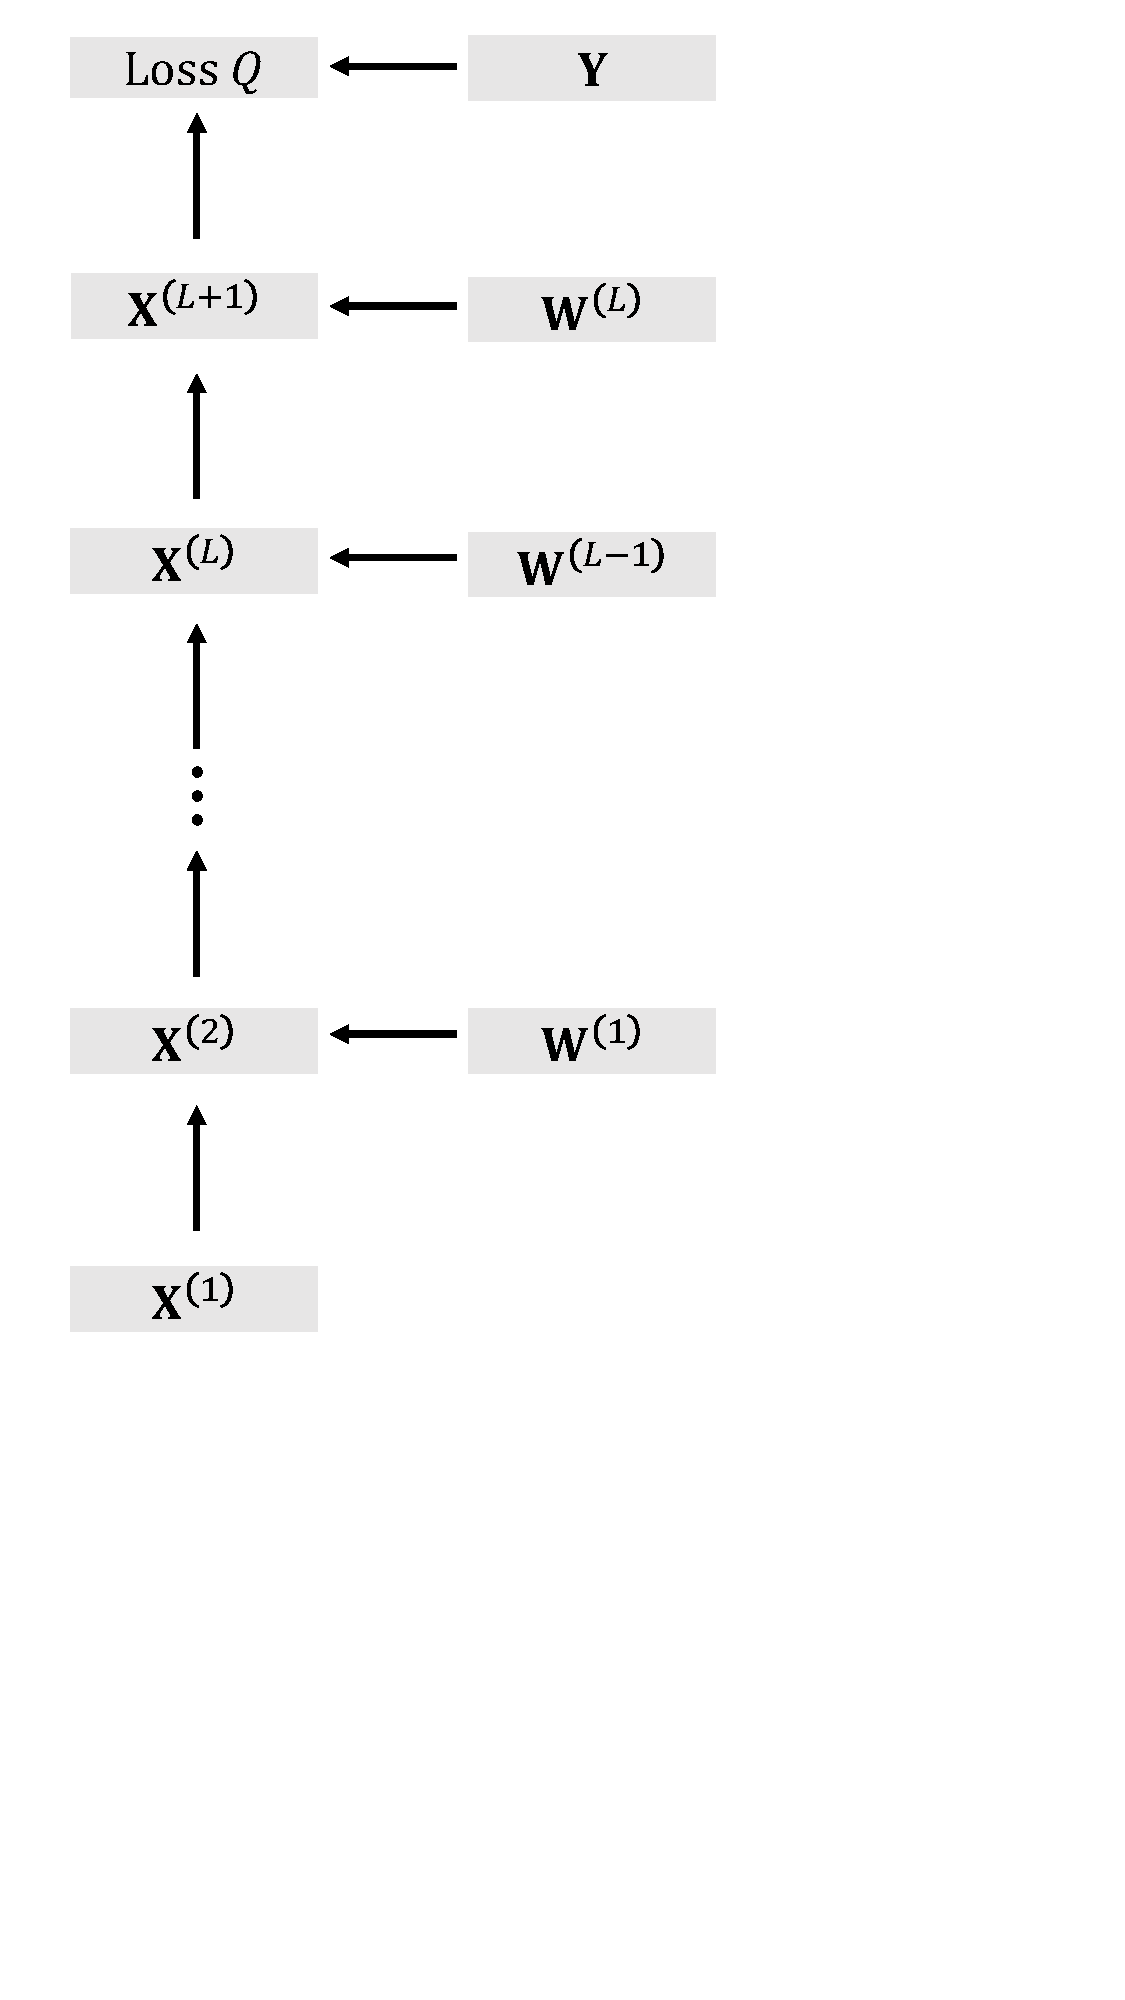
\includegraphics[width=0.3\textwidth]{figures/bp1.pdf}~~~
% 	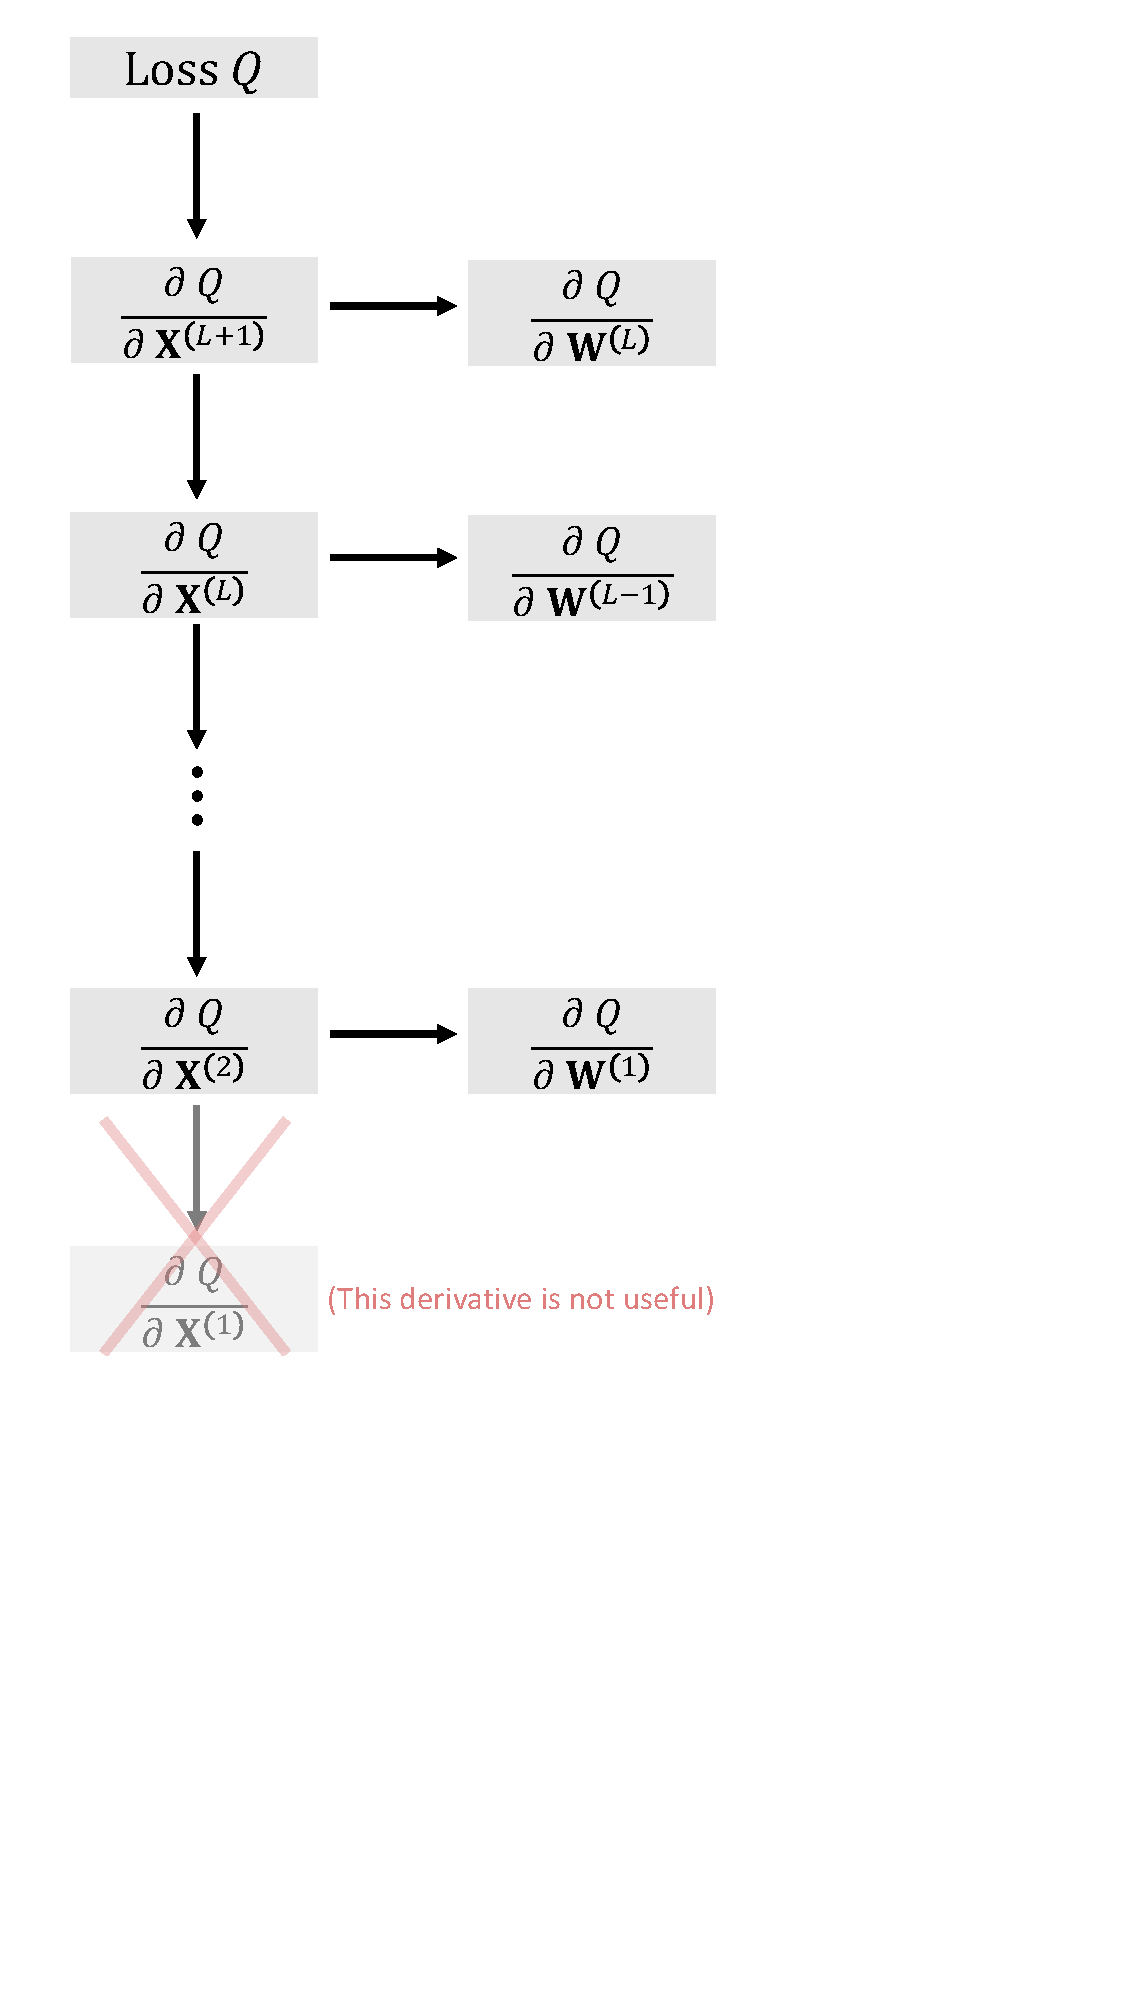
\includegraphics[width=0.3\textwidth]{figures/bp2.pdf}
% 	\caption{A}
% 	\label{fig:bp}
% \end{wrapfigure}


\begin{figure}[!h]
	\centering
	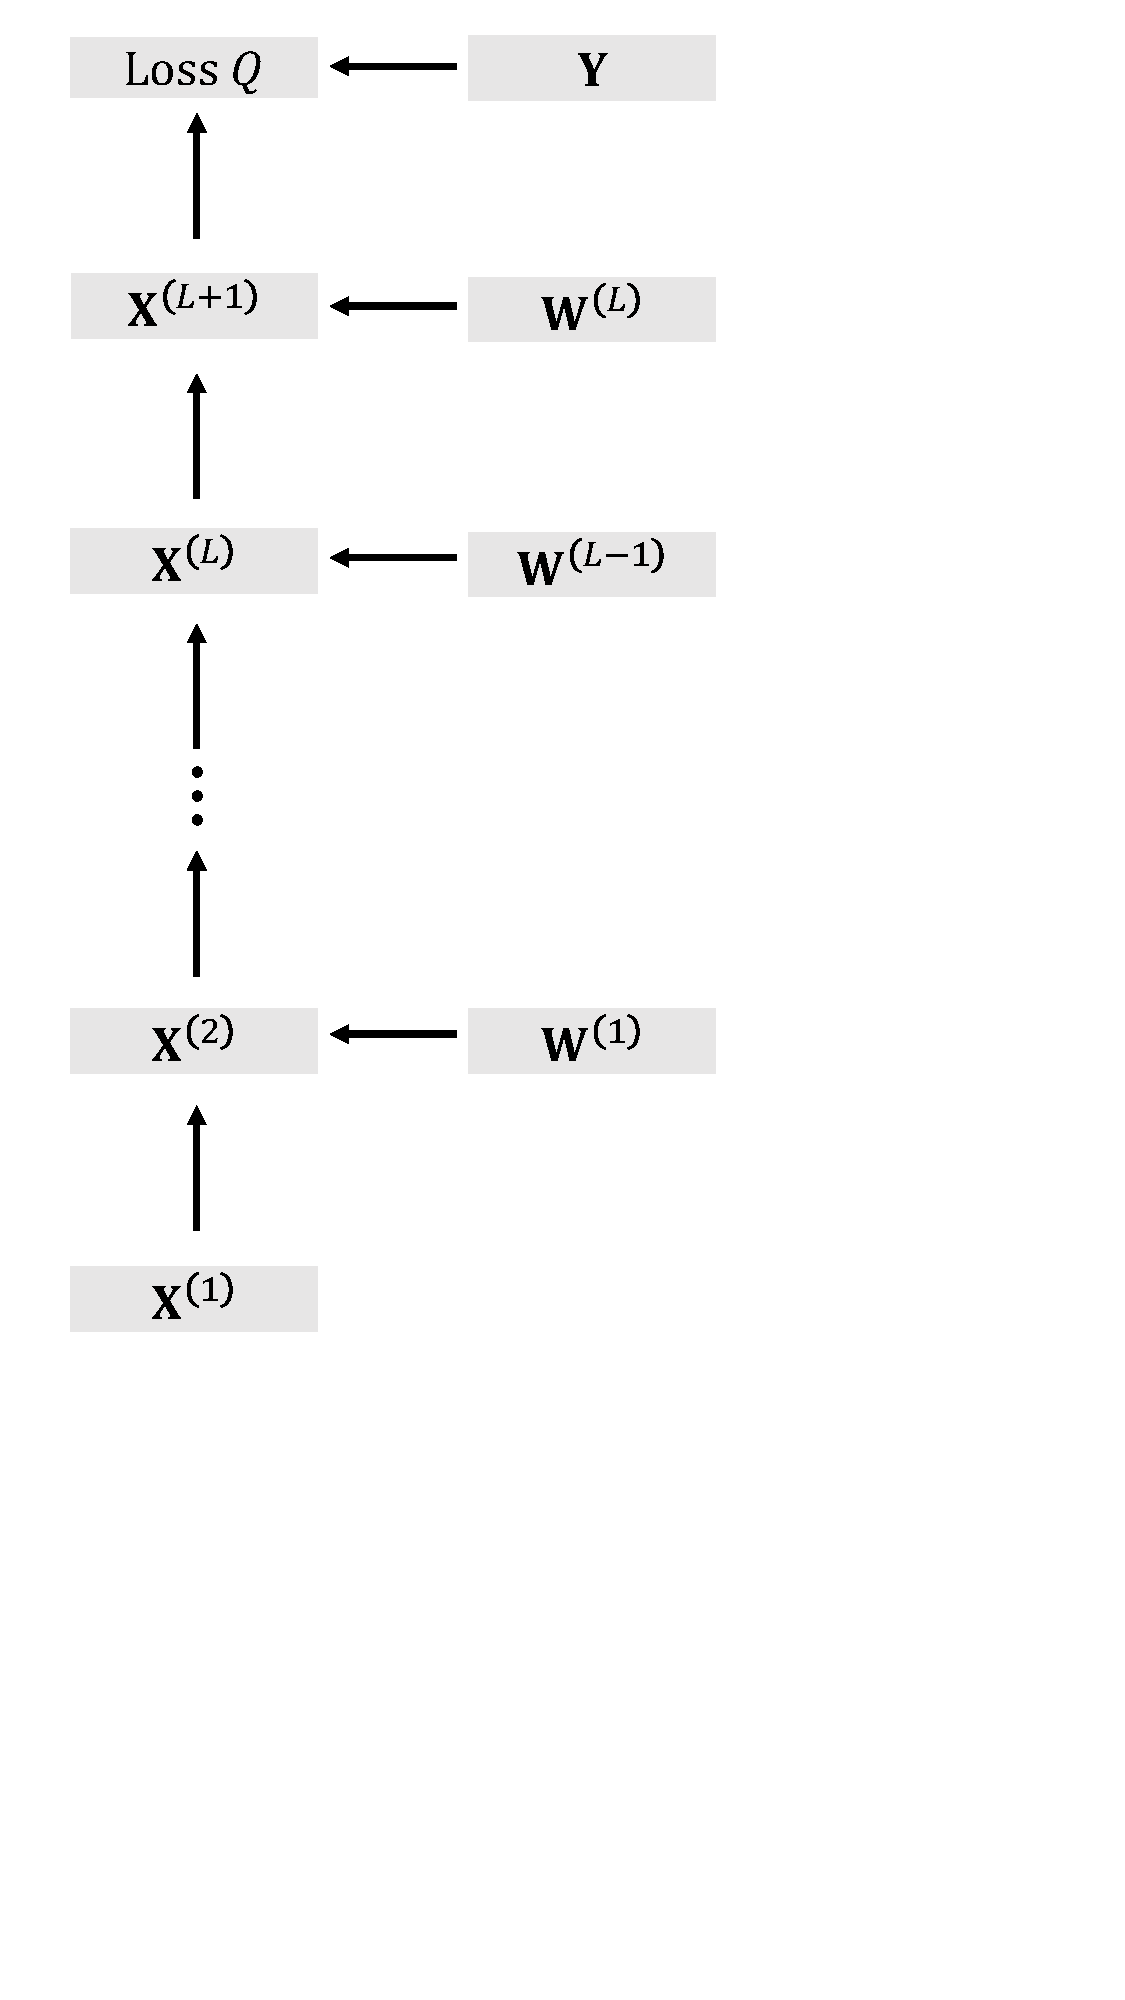
\includegraphics[width=0.35\linewidth]{figures/bp1.pdf}~~~~~~~~~~~~~~~~~~~~~~~~~~~~~~
	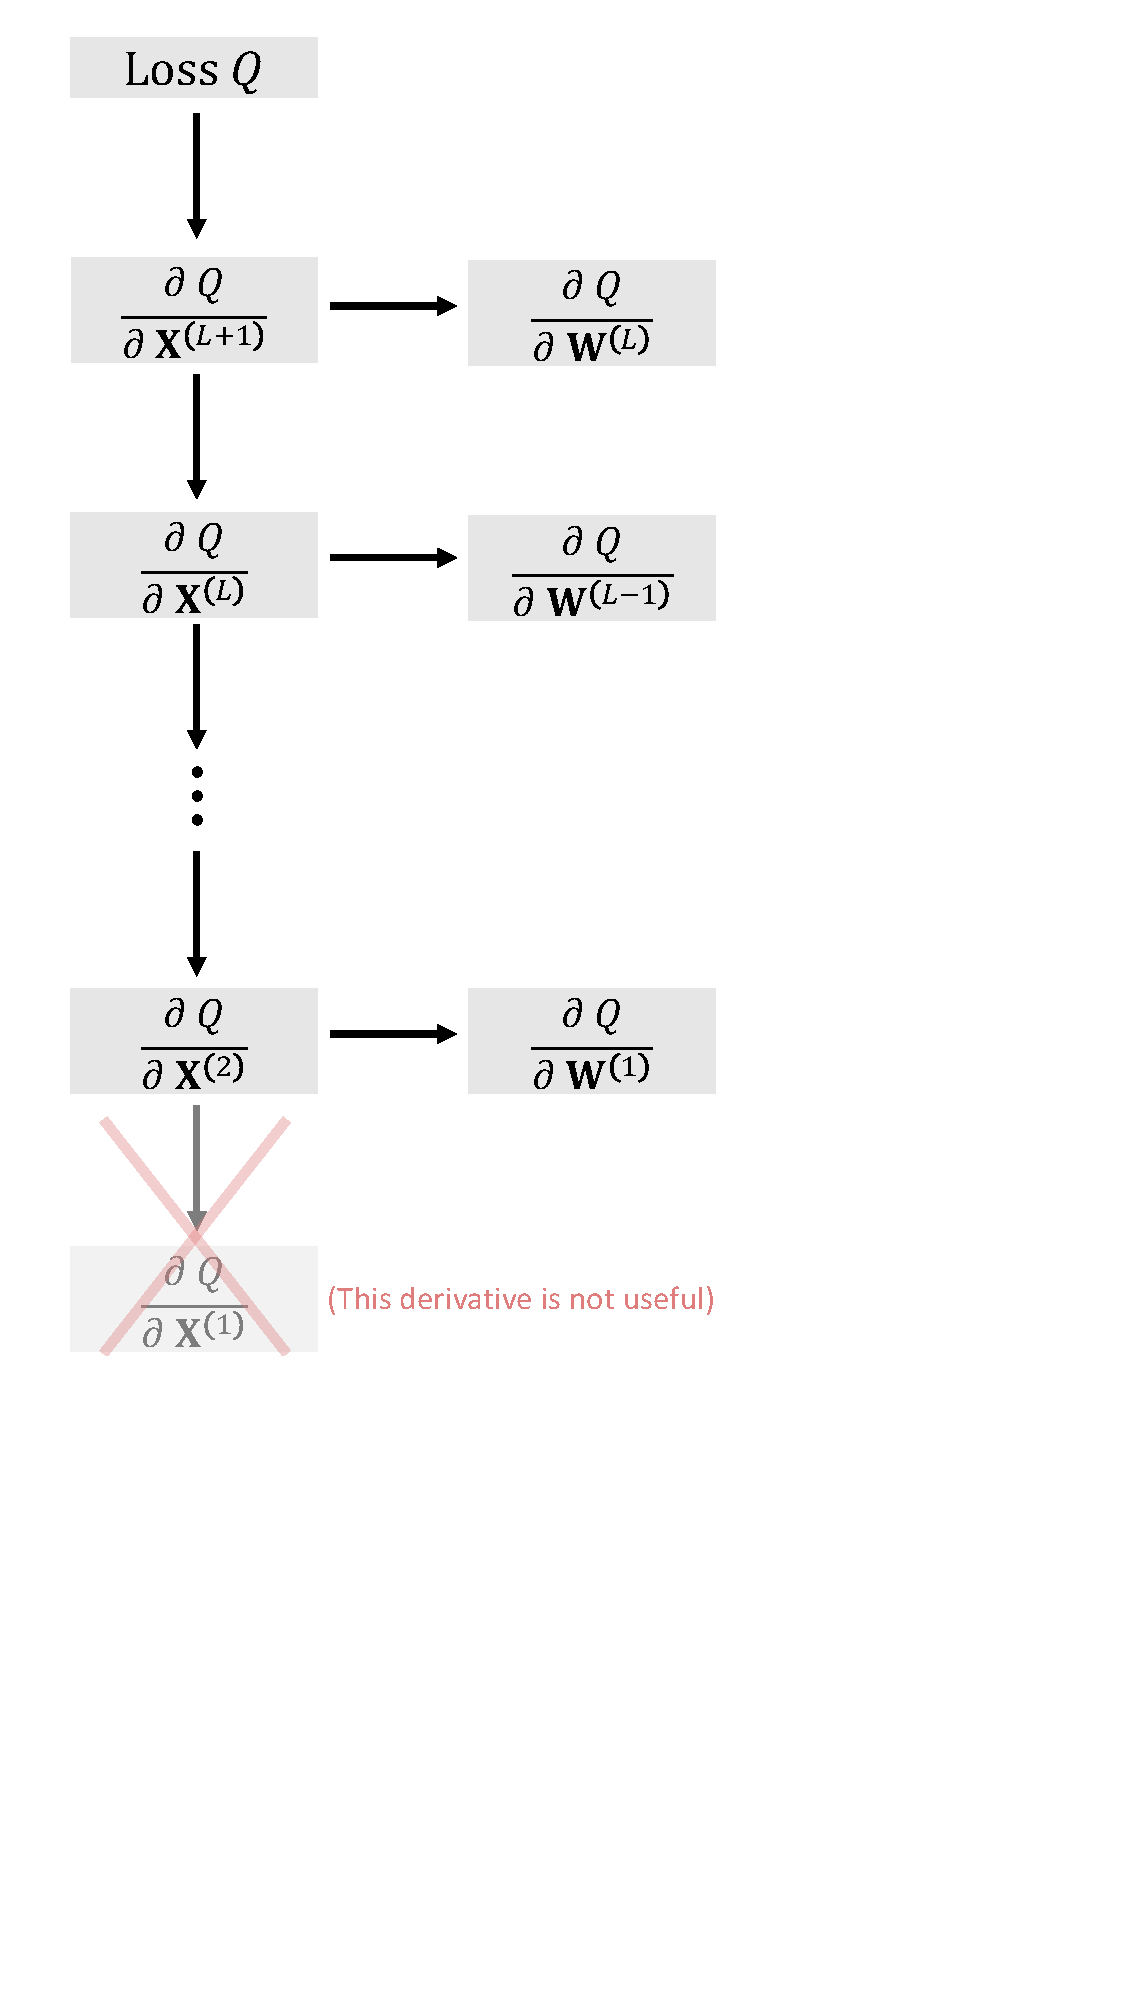
\includegraphics[width=0.35\linewidth]{figures/bp2.pdf}
	\caption{The forward and backward pass for computing gradients.}
	\label{fig:bp}
\end{figure}




\section{Computing Gradients via BackPropagation}

Let $Q$ be the loss function parameterized by $\W^{(1)}, \W^{(2)}, \cdots , \W^{(L)}$, where $\W^{(l)}$ is the weight of the $l$-th layer.
We seek to minimize $Q$ w.r.t.\ to the weights, so we need the gradients:
\begin{equation*}
    \frac{ \partial \, Q }{ \partial \, \W^{(1)} } , \; 
    \frac{ \partial \, Q }{ \partial \, \W^{(2)} } , \; \cdots , \;
    \frac{ \partial \, Q }{ \partial \, \W^{(L)} } .
\end{equation*}
With the gradients, we can update the weights $\W^{(1)}, \W^{(2)}, \cdots , \W^{(L)}$, e.g., by (stochastic) gradient descent:
\begin{equation} \label{eq:sgd}
    \W^{(l)} \: \longleftarrow \: \W^{(l)} - \alpha \, \frac{ \partial \, Q }{ \partial \, \W^{(l)} },
    \qquad \textrm{for } l=1, \cdots , L,
\end{equation}
where $\alpha$ ($>0$) is called step size or learning rate.
See my lecture note {\it Logistic Regression} for gradient-based algorithms.


Since $Q$ is complicated, directly computing $\frac{ \partial \, Q }{ \partial \, \W^{(l)} } $ for any layer is difficult.
The best practice is BackPropagation, that is, using the chain rule to let gradients flow from the top to the bottom.
See the illustration in Figure~\ref{fig:bp}(right).
\begin{itemize}
    \item 
    The loss function is a simple function of the output, $\X^{(L+1)}$.
    So it is easy to compute the derivative $\frac{\partial \, Q}{ \partial \, \X^{(L+1)}}$.
    \item
    After knowing $\frac{\partial \, Q}{ \partial \, \X^{(L+1)}}$, we can use the equations (chain rule) in Section~\ref{sec:differential} to compute 
    $\frac{\partial \, Q}{ \partial \, \W^{(L)}}$ and $\frac{\partial \, Q}{ \partial \, \X^{(L)}}$.
    We record $\frac{\partial \, Q}{ \partial \, \W^{(L)}}$ and pass $\frac{\partial \, Q}{ \partial \, \X^{(L)}}$ to the $(L-1)$-th layer.
    \item
    We repeat the above step from the $(L-1)$-th layer all the way down to the first (bottom) layer.
\end{itemize}
In this way, we obtained $\frac{ \partial \, Q }{ \partial \, \W^{(L)} } $, $\cdots$, $\frac{ \partial \, Q }{ \partial \, \W^{(2)} } $, $\frac{ \partial \, Q }{ \partial \, \W^{(1)} } $ one by one.
We will use them to update $\W^{(L)}$, e.g., according \eqref{eq:sgd}.




\section{Expressing Convolution as Matrix Multiplication}

The rest of this paper extends what we have done for FC layers to convolutional layers.
In this section, we express convolution as matrix multiplication to reveal the connection between FC layers and convolutional layers.
In the next section, we will derive the gradients for convolution.
Differentiation for convolutional layer is the same as FC layer except for the \textsf{unfold} and \textsf{fold} operations;
understanding \textsf{unfold} and \textsf{fold} will be the key to comprehend this and the next section.


\paragraph{Tensor convolution.}
Let $\T $ be a $d_1 \times d_2 \times d_3$ input tensor and $\K$ be a $k_1 \times k_2 \times d_3$ kernel (aka filter) tensor.
The convolution $\T * \K $ outputs a $(d_1 - k_1 + 1) \times (d_2 - k_2 + 1)$ matrix, denote $\C$.
\begin{itemize}
    \item 
    What decides the output shape of convolution? It is the number of $k_1 \times k_2 \times d_3$ patches in $\T$.
    Tensor $\T$ has $(d_1 - k_1 + 1) \times (d_2 - k_2 + 1)$ such patches.
    In Figure~\ref{fig:unfold}, since $d_1=4$, $d_2=3$, and $k_1=k_2=2$, there are totally $3\times 2 = 6$ patches.
    \item
    What are the entries of matrix $\C$?
    Let scalar $c_{ij} \in \RB$ be the $(i,j)$-th entry of $\C$ and tensor $\PP_{ij} \in \RB^{k_1 \times k_2 \times d_3}$ be the $(i,j)$-th patch of $\T$.
    Then
    \begin{equation}\label{eq:conv1}
        c_{ij} \: = \: \big\langle \K , \, \PP_{ij} \big\rangle
        \: = \:  \big\langle  \vect (\K) , \, \vect (\PP_{ij} )  \big\rangle .
    \end{equation}
    Here, $\vect (\K) $ means reshaping tensor $\K$ to a $k_1  k_2  d_3 \times 1$ vector, and $\langle \cdot , \cdot \rangle$ denotes vector/matrix/tensor inner product.
\end{itemize}


\paragraph{Unfolding.}
Based on the above discussions, we know that the $d_1 \times d_2 \times d_3$ tensor $\T $ can be converted to $(d_1 - k_1 + 1) \times (d_2 - k_2 + 1)$ patches;
each patch is a $k_1 \times k_2 \times d_3$ tensor (the same to the kernel $\K$).
Converting the order-3 tensor $\T$ to the order-5 tensor $\overline{\X}$ is called \textsf{unfolding}.
The shape of $\overline{\X}$ is
\begin{equation*}
    (d_1 - k_1 + 1) \times (d_2 - k_2 + 1) \times k_1 \times k_2 \times d_3;
\end{equation*}
$\overline{\X}$ consists of the patches $\{\PP_{ij}\}$:
\begin{equation*}
    \overline{\X} \, [i, \, j, \, :, \, :, \, :] \: = \: \PP_{ij} \: \in \: \RB^{k_1 \times k_2 \times d_3}.
\end{equation*}
Note that $\textsf{unfold}$ is supported by software systems like PyTorch.
Then, we \textsf{reshape} the order-5 tensor $\overline{\X}$ to the
\begin{equation*}
     (d_1 - k_1 + 1)  (d_2 - k_2 + 1)  \; \times \; (k_1 k_2 d_3 )
\end{equation*}
matrix, denote $\X$.
In sum, the procedure is
\begin{equation*}
    \T \textsf{ (order-3 tensor)}
    \: \xrightarrow{\textsf{unfold}} \:
    \overline{\X} \textsf{ (order-5 tensor)}
    \: \xrightarrow{\textsf{reshape}} \:
    \X \textsf{ (matrix)} .
\end{equation*}
Figure~\ref{fig:unfold} illustrates this procedure.

\paragraph{Convolution as matrix-vector multiplication.}
Let matrix $\X$ be the outcome after unfolding and reshaping.
Let $\w = \vect (\K) \in \RB^{k_1 k_2 d_3 \times 1}$ be the vectorization of $\K \in \RB^{k_1 \times k_2 \times d_3}$.
Then, compute the vector
\begin{equation} \label{eq:conv_multiply}
    \z \: = \: \X \, \cdot \, \vect (\K) 
    \: \in \: \RB^{ (d_1 - k_1 + 1)  (d_2 - k_2 + 1)  \times 1} .
\end{equation}
Recall that the $(d_1 - k_1 + 1) \times (d_2 - k_2 + 1)$ matrix $\C$ is the outcome of convolution.
By comparing \eqref{eq:conv1} and \eqref{eq:conv_multiply}, we find that
\begin{equation*}
    \z \: = \: \vect (\C )
    \qquad \textrm{and} \qquad
    \C \: = \: \textsf{reshape} \Big( \z , \, \big( (d_1 - k_1 + 1), (d_2 - k_2 + 1) \big) \Big) .
\end{equation*}
To summarize, the forward pass of tensor convolution can be expressed in the following two equivalent forms:
\begin{equation*}
    \left.
    \begin{array}{c}
         \T \textsf{ (input tensor)} \\
         \K \textsf{ (kernel tensor)} \\
    \end{array}
    \right\}
    \: \xrightarrow{\textsf{convolution}}  \: 
    \C  \textsf{ (output matrix)} 
\end{equation*}
and
\begin{equation} \label{eq:conv2}
    \left.
    \begin{array}{r c}
         \T \: \xrightarrow{\textsf{unfold}} \: \overline{\X} \: \xrightarrow{\textsf{reshape}}  & \X \\
         \K \: \xrightarrow{\textsf{vectorize}} & \w  \\
    \end{array}
    \right\}
    \: \xrightarrow{\textsf{multiply}}  \: 
    \z
    \: \xrightarrow{\textsf{reshape}}  \: 
    \C .
\end{equation}
In the next section, we will use the latter to perform backpropagation.



\begin{figure}[!h]
	\centering
	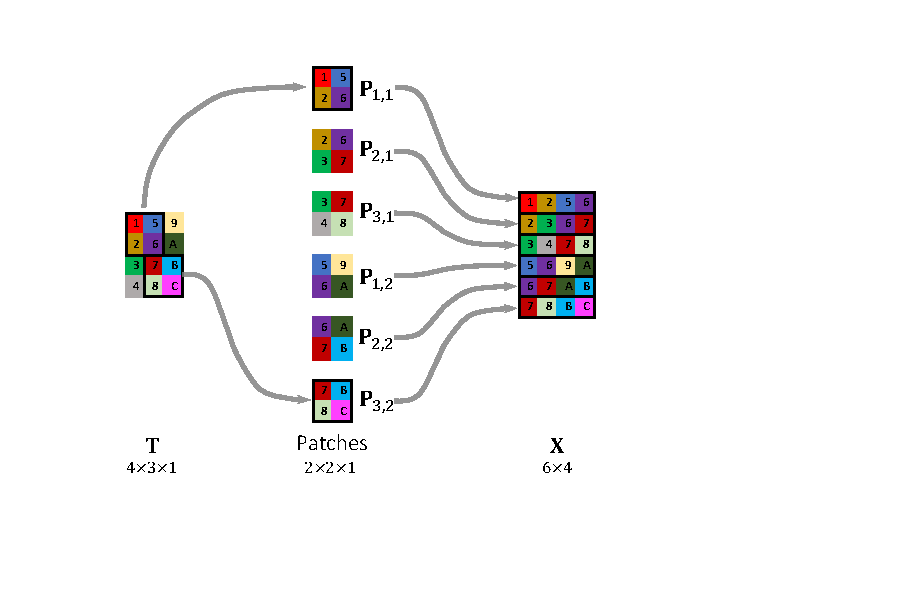
\includegraphics[width=0.7\linewidth]{figures/unfold.pdf}
	\caption{Illustrating patching and unfolding. Here, $d_1=4$, $d_2=3$, $d_3=1$, and $k_1=k_2=2$.
	Thus, there are $(d_1-k_1+1)\times (d_2-k_2+1) = 6$ patches, and each patch is $k_1\times k_2 = 2\times 2$.}
	\label{fig:unfold}
\end{figure}

\section{Differentiation for Convolution}


By representing convolution as the procedure \eqref{eq:conv2}, the backpropagation will be easier to derive.
During the backpropagation, we receive $\frac{\partial \, Q}{\partial \, \C}$ and propagate it to $\K$ and $\T$.
The backpropagation has the following steps:
\begin{equation} \label{eq:conv2}
    \left.
    \begin{array}{r c}
         \frac{\partial \, Q}{\partial \, \T} \: \xleftarrow{\textsf{fold}} \: \frac{\partial \, Q}{\partial \, \overline{\X}} \: \xleftarrow{\textsf{reshape}}  & \frac{\partial \, Q}{\partial \, \X} \\
         \frac{\partial \, Q}{\partial \, \K} \: \xleftarrow{\textsf{reshape}} & \frac{\partial \, Q}{\partial \, \w}  \\
    \end{array}
    \right\}
    \: \xleftarrow{\textsf{multiply}}  \: 
    \frac{\partial \, Q}{\partial \, \z}
    \: \xleftarrow{\textsf{vectorize}}  \: 
    \frac{\partial \, Q}{\partial \, \C} .
\end{equation}
We describe the steps one by one.


\paragraph{From $\C$ to $\z$.}
This step is almost trivial.
Since $\z = \vect (\C)$, we have
\begin{equation*}
    \frac{\partial \, Q}{\partial \, \z}
    \: = \: \vect \left( \frac{\partial \, Q}{\partial \, \C} \right) 
    \: \in \: \RB^{(d_1-k_1+1)(d_2-k_2+1) \times 1} .
\end{equation*}
It just performs a vectorization.



\paragraph{From $\z$ to $\X$ and $\w$.}
Recall from \eqref{eq:conv_multiply} that $\z$ is computed by the matrix-vector multiplication: $\z= \X \w$.
Once we have $\frac{ \partial \, Q}{\partial \, \z}$, we can propagate it to $\X$ and $\w$ by
\begin{align*}
    & \underbrace{\frac{ \partial \, Q }{ \partial \, \X } }_{(d_1 - k_1 + 1)  (d_2 - k_2 + 1)  \times (k_1 k_2 d_3)}
    \: = \: \underbrace{\frac{ \partial \, Q }{ \partial \, \z } }_{(d_1 - k_1 + 1)  (d_2 - k_2 + 1)  \times 1}
    \underbrace{\w^T }_{ 1 \times (k_1 k_2 d_3)} ,\\
    & \underbrace{ \frac{ \partial \, Q }{ \partial \, \w } }_{ (k_1 k_2 d_3) \times 1} 
    \: = \:\underbrace{\X^T }_{(k_1 k_2 d_3) \times (d_1 - k_1 + 1)  (d_2 - k_2 + 1)}
    \underbrace{\frac{ \partial \, Q }{ \partial \, \z } }_{(d_1 - k_1 + 1)  (d_2 - k_2 + 1)  \times 1} .
\end{align*}
The above equations follow from \eqref{eq:grad_q_x} and \eqref{eq:grad_q_w}.


\paragraph{From $\w$ to $\K$.}
Since $\w = \vect (\K) $, the $k_1\times k_2 \times d_3$ tensor $\K$ can be obtained by \textsf{reshaping} $\w$ to order-3 tensor.
Thus,
\begin{equation*}
    \frac{ \partial \, Q }{ \partial \, \K } \:= \: 
    \textsf{reshape} \left( \frac{\partial \, Q}{\partial \, \w}  \; , \Big( k_1, \,  \, k_2 , \, d_3 \Big)  \right)
\end{equation*}

\paragraph{From $\X$ to $\T$.}
As illustrated in Figure~\ref{fig:unfold}, $\X$ is obtained by \textsf{unfolding} $\T$,
and one entry of $\T$ is copied to multiple (at most $k_1k_2$) entries of $\X$.
For example, in Figure~\ref{fig:unfold}, the \textcolor{OliveGreen}{green ``A''} entry is copied from $t_{2,3,1}$ to both $x_{4,4}$ and $x_{5,3}$.\footnote{We let $x_{ij} = \X[i,j]$ denote the $(i,j)$-th entry of $\X$.}
Thus
\begin{equation} \label{eq:t_x_1}
     \textcolor{OliveGreen}{t_{2,3,1}} 
     \: = \: 
     \textcolor{OliveGreen}{x_{4,4}} 
     \: = \: 
     \textcolor{OliveGreen}{x_{5,3}} .
\end{equation}
So the $(2,3,1)$-th entry of $\T$ influences $Q$ via only two enties of $\X$, and thus
\begin{equation*}
    \frac{\partial \, x_{ij}}{\partial \, t_{2,3,1}} 
    \: = \:
    \left\{
    \begin{array}{c l}
         1 & \textrm{if } (i,j)=(4,4) \textrm{ or } (5,3);  \\
         0 & \textrm{otherwise}. \\ 
    \end{array}
    \right.
\end{equation*}
It follows that
\begin{equation} \label{eq:t_x_2}
    \bigg[\frac{\partial \, Q}{\partial \, \T} \bigg]_{2, 3, 1}
    \: = \: \sum_{i, j}  \frac{\partial \, x_{ij}}{\partial \, t_{2,3,1}} \, \frac{\partial \, Q}{\partial \, x_{ij}} 
    \: = \: \frac{\partial \, Q}{\partial \, x_{4,4}} + \frac{\partial \, Q}{\partial \, x_{5,3}}  
    \: = \: \bigg[\frac{\partial \, Q}{\partial \, \X} \bigg]_{4, 4} \, + \,\bigg[ \frac{\partial \, Q}{\partial \, \X} \bigg]_{5, 3} . 
\end{equation}
Deep learning platforms like PyTorch provide the ``\textsf{fold}'' for aggregating the entries of $\frac{\partial \, Q}{\partial \, \X} $ to get $\frac{\partial \, Q}{\partial \, \T}$.\footnote{The aggregation is according to the way the entries of $\T$ are copied to $\X$, e.g., $t_{2,3,1}$ is copied to $x_{4,4}$ and $x_{5,3}$.}
First, \textsf{reshape} $\frac{\partial \, Q}{\partial \, \X} $ to the $(d_1 - k_1 + 1) \times (d_2 - k_2 + 1) \times k_1 \times k_2 \times d_3$ order-5 tensor:
\begin{equation*}
    \frac{\partial \, Q}{\partial \, \overline{\X}}  \:= \: \textsf{reshape} \left( \frac{\partial \, Q}{\partial \, \X}  \; , \Big( (d_1 - k_1 + 1) , \, (d_2 - k_2 + 1) , \, k_1 , \, k_2 , \, d_3 \Big)  \right) .
\end{equation*}
Then, apply ``\textsf{fold}'' to get the $d_1\times d_2 \times d_3$ order-3 tensor  $\frac{\partial \, Q}{\partial \, \T}$:
\begin{equation*}
    \frac{\partial \, Q}{\partial \, \T}
    \: = \: \textsf{fold} \left( \frac{\partial \, Q}{\partial \, \overline{\X}}   \right).
\end{equation*}
To summerize, the forward pass from $\T$ to $\X$ and the backward pass from $\X$ to $\T$ are
\begin{equation*}
    \T \: \xrightarrow{\textsf{unfold}} \: \overline{\X} \: \xrightarrow{\textsf{reshape}}  \: \X
    \qquad \textrm{and} \qquad
    \frac{\partial \, Q}{\partial \, \T} 
    \: \xleftarrow{\textsf{~fold~}} \: 
    \frac{\partial \, Q}{\partial \, \overline{\X}} 
    \: \xleftarrow{\textsf{reshape}}  \: 
    \frac{\partial \, Q}{\partial \, \X} .
\end{equation*}








\end{document}
